% \begin{figure}[t]
\begin{small}
\begin{center}
\begin{tabular}{|l|c|c|c|c|} \hline \T
Config.                & \multicolumn{2}{c|}{Throughput (MB/s)}  & \multicolumn{2}{c|}{Latency (ms)} \\ \cline{2-5}
                       & Median   & Quartiles \T                 & Median & Quartiles                \\ \hline \T
\JikesRVM{}            & 122.437  & 121.44--123.32               & 0.442  & 0.394--0.496             \\
\DSU{}                 & 121.308  & 121.12--121.41               & 0.349  & 0.341--0.351             \\
\DSU{} upd             & 121.242  & 121.09--121.29               & 0.345  & 0.341--0.349             \\ \hline
\end{tabular}
\end{center}
\end{small}
% \caption{Throughput and latency measurements for Jetty webserver v5.1.6
% showing median and semi-interquartile range\label{tab:jetty}}
\begin{center}
\scalebox{0.63}{\includegraphics{graphs/jetty-throughput-latency}}
\caption{Throughput and latency measurements of Jetty webserver v5.1.6\label{fig:jetty}}
\end{center}
\end{figure}

% \begin{figure}[t]
\begin{center}
\scalebox{0.63}{\includegraphics{graphs/jetty-throughput-latency}}
\caption{Throughput and latency measurements of Jetty webserver v5.1.6\label{fig:jetty}}
\end{center}
\end{figure}

% \begin{table*}[t]
\begin{footnotesize}
\begin{center}
\begin{tabular}{|r|r|rrrrrrrrrrr|}
                                                                                                                                   \hline
\multirow{2}{*}{\# objects}     & \multicolumn{1}{c}{Heap}   & \multicolumn{11}{|c|}{Fraction of updated objects \T}            \\
                                & \multicolumn{1}{c|}{size}  &
                       0\%  &   10\%  &   20\%  &   30\%  &   40\%  &   50\%  &   60\%  &   70\%  &   80\%  &   90\%  &  100\%  \\ \hline
\multicolumn{13}{|c|}{Garbage collection time (ms) \T}                                                                          \\ \hline \T
 280000 &  160 MB &    78.2 &    81.3 &    83.1 &    89.3 &    99.0 &   103.2 &   108.3 &   113.2 &   113.3 &   120.3 &   120.0 \\
 770000 &  320 MB &   148.9 &   165.0 &   181.9 &   195.8 &   213.2 &   223.2 &   237.0 &   249.0 &   262.0 &   269.5 &   278.6 \\
1760000 &  640 MB &   313.3 &   347.7 &   382.9 &   416.0 &   449.8 &   478.9 &   506.8 &   534.0 &   558.8 &   583.7 &   601.5 \\
3670000 & 1280 MB &   615.4 &   694.6 &   763.0 &   833.6 &   900.1 &   965.9 &  1019.0 &  1076.4 &  1129.9 &  1181.2 &  1217.5 \\ \hline
\multicolumn{13}{|c|}{Running transformation functions (ms) \T}                                                                 \\ \hline \T
 280000 &  160 MB &     0.1 &    13.0 &    23.2 &    34.6 &    43.9 &    54.0 &    62.7 &    74.5 &    84.1 &    93.9 &   104.2 \\
 770000 &  320 MB &     0.1 &    33.7 &    63.1 &    91.2 &   116.8 &   145.4 &   173.9 &   201.0 &   231.3 &   262.0 &   292.6 \\
1760000 &  640 MB &     0.1 &    77.9 &   143.9 &   207.7 &   269.5 &   333.7 &   397.6 &   464.0 &   534.6 &   604.5 &   674.9 \\
3670000 & 1280 MB &     0.1 &   160.8 &   299.2 &   429.4 &   560.2 &   693.8 &   827.3 &   975.0 &  1119.6 &  1263.7 &  1405.4 \\ \hline
\multicolumn{13}{|c|}{Total DSU pause time (ms) \T}                                                                             \\ \hline \T
 280000 &  160 MB &    82.8 &    99.0 &   109.5 &   128.0 &   147.6 &   161.2 &   174.5 &   192.8 &   202.5 &   218.8 &   228.1 \\
 770000 &  320 MB &   153.6 &   202.9 &   249.0 &   291.4 &   334.5 &   372.6 &   414.8 &   455.4 &   498.1 &   535.3 &   576.8 \\
1760000 &  640 MB &   316.6 &   429.5 &   530.5 &   627.2 &   723.4 &   816.0 &   908.6 &  1002.6 &  1097.5 &  1191.5 &  1281.2 \\
3670000 & 1280 MB &   618.7 &   859.0 &  1065.9 &  1269.9 &  1466.1 &  1663.6 &  1850.8 &  2054.2 &  2253.1 &  2448.5 &  2627.9 \\ \hline
\end{tabular}
\end{center}
\end{footnotesize}
\caption{Microbenchmark results: \DSU{} update pause time (in ms) for various heap sizes}
\label{tab:microbench}
\end{table*}


\begin{figure}[t]
\centering
\begin{small}
\begin{tabular}{lcccc} \toprule
\multirow{2}{*}{Config.} & \mc{2}{c}{Throughput (MB/s)}  & \mc{2}{c}{Latency (ms)} \\ \cmidrule{2-5}
           & Median   & Quartiles                    & Median & Quartiles     \\ \midrule
%            & \mc{2}{c}{Throughput (MB/s)}  & \mc{2}{c}{Latency (ms)} \\ \cmidrule{2-5}
% Config.    & Median   & Quartiles                    & Median & Quartiles     \\ \midrule
\RVM       & 122.437  & 121.44--123.32               & 0.442  & 0.394--0.496  \\
\JV        & 121.308  & 121.12--121.41               & 0.349  & 0.341--0.351  \\
\JV upd.   & 121.242  & 121.09--121.29               & 0.345  & 0.341--0.349  \\ \bottomrule
\end{tabular}
\end{small}
\\[2ex]
\includegraphics[scale=0.63]{100-graphs/jetty-throughput-latency}
% \caption{Throughput and latency measurements of Jetty webserver v5.1.6\label{fig:jetty}}
\hangcaption{Throughput and latency measurements for Jetty webserver
version 5.1.6 showing median and semi-interquartile range\label{fig:jetty}}
\VspaceFixForHangcaption
\end{figure}

% vim:tw=0


\subsection{Jetty Webserver performance}
\label{subsec:jetty-webserver-performance}

To see the effect of updating on application performance, we measured Jetty
under various request rates using httperf\index{httperf}, a webserver
benchmarking tool~\cite{httperf}, and determined Jetty's saturation rate to
be roughly 800 new connection requests/second. We then measured Jetty's
performance by issuing connections at this rate.  Each connection makes 5
serial requests for a 40 Kbyte file. Httperf reports average throughput and
average per-request latency over a 60 second period. We ran this experiment
21 times and report the median and quartiles of the throughput and latency
reports. With 21 runs, the range between the quartiles serves as a 98\%
confidence interval~\cite{PrattGibbons81}. In order to eliminate network
traffic effects, we ran the server on two cores of a quad-core machine and
the client on another core.

Figure~\ref{fig:jetty} shows our results in tabular form and plotted
graphically.  The second and third columns of the table report the median
throughput and the range between the two quartiles.  The third column and
fourth column report the median latency and the inter-quartile range.  The
first and second rows illustrate the performance of Jetty version 5.1.6
running on stock \RVM and \JV, respectively. The third row shows the
performance on \JV of Jetty 5.1.6 dynamically updated from version 5.1.5
prior to the start of the experiment.  The performance of the two \JV
configurations are statistically indistinguishable.  The two configurations'
corresponding inter-quartile ranges largely overlap.  The performance of
\JV is also quite similar to the performance of stock \RVM.  There are many
small differences between \JV and the stock implementation that change VM
code size, code layout, and garbage collection behavior. These differences
may impact performance directly and they may indirectly affect other
elements of the VM, such as the timing of garbage collections and JIT
optimizations (such indirect effects make VMs notoriously difficult to
benchmark~\cite{dacapo-cacm, diwan-measurement}).
